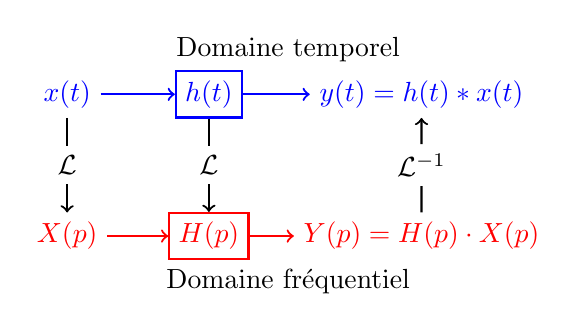
\begin{tikzpicture}

\begin{scope}[local bounding box=diagramme, scale=0.9, anchor=center, baseline]
    \node[blue] (x) at (0, 2) {$x(t)$};
    \node [draw, rectangle, thick, color=blue] (h) at (2, 2) {$h(t)$};
    \node[blue] (y) at (5, 2) {$y(t) = h(t) * x(t)$};
    \draw[->, thick, blue] (x) -- (h);
    \draw[->, thick, blue] (h) -- (y);
    
    \node (laplace1) at (0, 1) {$\mathcal{L}$};
    \node (laplace2) at (2, 1) {$\mathcal{L}$};
    \node (inverse_laplace) at (5, 1) {$\mathcal{L}^{-1}$};
    \draw[thick] (x) -- (laplace1);
    \draw[thick] (h) -- (laplace2);
    \draw[<-, thick] (y) -- (inverse_laplace);
    
    \node[red] (X) at (0, 0) {$X(p)$};
    \node [draw, rectangle, thick, color=red] (H) at (2, 0) {$H(p)$};
    \node[red] (Y) at (5, 0) {$Y(p) = H(p) \cdot X(p)$};
    \draw[->, thick, red] (X) -- (H);
    \draw[->, thick, red] (H) -- (Y);
    
    \draw[->, thick] (laplace1) -- (X);
    \draw[->, thick] (laplace2) -- (H);
    \draw[thick] (inverse_laplace) -- (Y);
\end{scope}
\node at (diagramme.north) [above] {Domaine temporel};
\node at (diagramme.south) [below] {Domaine fréquentiel};
    
\end{tikzpicture}